\documentclass[11pt,a4paper]{article}

\usepackage[margin=1in]{geometry}
\usepackage{amsmath,amsthm,amssymb,mathtools}
\usepackage{enumitem}
\usepackage{booktabs}
\usepackage{hyperref}
\usepackage{xcolor}
\usepackage[utf8]{inputenc}
\usepackage{listings}
\usepackage{array}
\usepackage{tikz}
\usetikzlibrary{arrows.meta,positioning,calc,decorations.pathreplacing}

\lstset{
  language={},
  basicstyle=\small\ttfamily,
  keywordstyle=\bfseries,
  commentstyle=\itshape\color{gray},
  breaklines=true,
  frame=single,
  numbers=none,
  xleftmargin=1em,
  literate=
    {negation}{{\ensuremath{\neg}}}1
    {forall}{{\ensuremath{\forall}}}1
    {exists}{{\ensuremath{\exists}}}1
    {->}{{\ensuremath{\to}}}2
    {<-}{{\ensuremath{\leftarrow}}}2
    {/\\}{{\ensuremath{\land}}}2
    {\\/}{{\ensuremath{\lor}}}2
    {>=}{{\ensuremath{\geq}}}2
    {<=}{{\ensuremath{\leq}}}2
    {!=}{{\ensuremath{\neq}}}2
    {*}{{\ensuremath{\times}}}1,
}

%% ---- Theorem environments ----
\newtheorem{theorem}{Theorem}[section]
\newtheorem{lemma}[theorem]{Lemma}
\newtheorem{proposition}[theorem]{Proposition}
\newtheorem{corollary}[theorem]{Corollary}
\theoremstyle{definition}
\newtheorem{definition}[theorem]{Definition}
\newtheorem{example}[theorem]{Example}
\theoremstyle{remark}
\newtheorem{remark}[theorem]{Remark}

%% ---- Macros ----
\newcommand{\BISH}{\mathrm{BISH}}
\newcommand{\LPO}{\mathrm{LPO}}
\newcommand{\LLPO}{\mathrm{LLPO}}
\newcommand{\WLPO}{\mathrm{WLPO}}
\newcommand{\MP}{\mathrm{MP}}
\newcommand{\CLASS}{\mathrm{CLASS}}
\newcommand{\DPT}{\mathrm{DPT}}
\newcommand{\Qp}{\mathbb{Q}_p}
\newcommand{\Fp}{\mathbb{F}_p}
\newcommand{\Dcris}{D_{\mathrm{cris}}}
\newcommand{\Dst}{D_{\mathrm{st}}}
\newcommand{\DdR}{D_{\mathrm{dR}}}
\newcommand{\NM}{N_M}
\newcommand{\vp}{v_p}
\newcommand{\Ext}{\mathrm{Ext}}
\newcommand{\CH}{\mathrm{CH}}
\newcommand{\Sha}{\mathrm{III}}
\newcommand{\leanRepo}{\url{https://doi.org/10.5281/zenodo.18735931}}


\title{\textbf{De Rham Decidability and DPT Completeness} \\[4pt]
\large The $p$-adic Precision Bound \\[4pt]
\normalsize Paper~59/60, Constructive Reverse Mathematics Series}

\author{Paul Chun-Kit Lee\\New York University, Brooklyn, NY\footnote{Lean~4 source code and reproducibility materials: \leanRepo}}

\date{February 2026}

\begin{document}
\maketitle

%% ===================================================================
\begin{abstract}
%% ===================================================================

We formalize the $p$-adic precision bound $\NM = \vp(\det(1 - \varphi))$
for elliptic curves with good reduction.  The key identity
\[
  \NM = \vp(1 - a_p + p) = \vp(\#E(\Fp))
\]
shows that the precision lost in $p$-adic verification equals the $p$-adic
valuation of the point count on the reduction.  The Hasse bound
$a_p^2 \le 4p$ implies $\#E(\Fp) \ge 1$, so $\NM$ is always well-defined.

We verify $\NM$ for 24 entries across 4 elliptic curves
($X_0(11)$, $X_0(14)$, $X_0(15)$, 37a) at primes of good reduction.
Four entries are anomalous ($\NM \ge 1$); the remaining 20 are generic ($\NM = 0$):

\smallskip
\begin{center}
\begin{tabular}{ccccl}
\toprule
Curve & $p$ & $\det(1{-}\varphi)$ & $\NM$ & Note \\
\midrule
$X_0(11)$ & 5 & 5 & 1 & $5 \mid 5$ \\
$X_0(14)$ & 3 & 6 & 1 & $3 \mid 6$, $9 \nmid 6$ \\
$X_0(15)$ & 2 & 4 & 2 & Max $\NM$ in table \\
$X_0(15)$ & 7 & 7 & 1 & $7 \mid 7$, $49 \nmid 7$ \\
\bottomrule
\end{tabular}
\end{center}
\smallskip

\noindent ``Axiom~5'' (de Rham decidability) is a theorem for geometric representations:
de Rham (Faltings/Tsuji) $\Rightarrow$ potentially semistable (Berger) $\Rightarrow$
weakly admissible (Colmez--Fontaine) $\Rightarrow$ $\NM$ computable in $\BISH$.

\medskip
\noindent\textbf{CRM classification:} $\BISH$.  All arithmetic is exact over~$\mathbb{Z}$; no omniscience principles invoked.

\medskip
\noindent\textbf{Lean~4 formalization:} 6~modules (${\sim}762$ lines), zero errors, zero warnings, zero sorry.  Zero custom axioms; all precision bounds verified by \texttt{norm\_num} and \texttt{simp}.
\end{abstract}


%% ===================================================================
\section{Introduction}
\label{sec:intro}
%% ===================================================================

\subsection{Main results}
\label{sec:main-results}

This paper quantifies the $p$-adic precision cost of de Rham verification for elliptic curves with good reduction.  The entire computation is pure integer arithmetic: no $p$-adic analysis or period rings appear in the Lean formalization.

\begin{enumerate}[label=\textbf{(\Alph*)}]
\item \textbf{Hasse implies positivity} (Theorem~\ref{thm:hasse_positive}).  For $p \ge 2$ with $a_p^2 \le 4p$: $1 - a_p + p > 0$.  Equivalently, $\#E(\Fp) \ge 1$, so $\NM$ is always well-defined.

\item \textbf{Ordinary, non-anomalous} (Theorem~\ref{thm:ordinary}).  If $p \nmid (1 - a_p)$, then $\NM = 0$: no precision loss.

\item \textbf{Supersingular, no precision loss} (Theorem~\ref{thm:supersingular}).  When $a_p = 0$: $\det(1-\varphi) = 1 + p$ and $\NM = 0$.

\item \textbf{Verification table} (\S\ref{sec:table}).  24 entries across 4 elliptic curves ($X_0(11)$, $X_0(14)$, $X_0(15)$, 37a).  Four anomalous ($\NM \ge 1$), 20 generic ($\NM = 0$).  Maximum $\NM = 2$ at $X_0(15)/p{=}2$.

\item \textbf{Semistable extension} (Theorem~\ref{thm:semistable}).  For split multiplicative reduction (Tate curves), $\NM^{\mathrm{st}} = \vp(q_E)$ is computable from the $j$-invariant.

\item \textbf{DPT completeness} (Theorem~\ref{thm:completeness}).
Axioms~1--3 plus de~Rham decidability suffice for the decidability of numerical equivalence on~$\CH^*(X)$.  No mixed motive axiom is needed: $\Ext^1$ is invisible to numerical equivalence.  The pure motive program (Papers~50--59) is complete.

\item \textbf{Analytic rank stratification} (Theorem~\ref{thm:rank-strat}).
The logical complexity of computing $\Ext^1(\mathbb{Q}(0), M)$ is stratified by the analytic rank $r = \mathrm{ord}_{s=s_0} L(M,s)$: $r = 0$ and $r = 1$ are $\BISH$; $r \ge 2$ requires~$\MP$.
\end{enumerate}


\subsection{Constructive reverse mathematics primer}
\label{sec:crm-primer}

Bishop-style constructive mathematics ($\BISH$)~\cite{Bishop1985} works within intuitionistic logic: no excluded middle, no axiom of choice.  Classical theorems are recovered by adding \emph{omniscience principles}:
\[
  \BISH \;\subset\; \BISH + \MP \;\subset\; \BISH + \LLPO \;\subset\; \BISH + \LPO \;\subset\; \CLASS.
\]
Constructive reverse mathematics (CRM) classifies theorems by the \emph{weakest} principle required.  This paper operates entirely in~$\BISH$: all arithmetic is exact over~$\mathbb{Z}$, all witnesses are explicit, and no omniscience principle is needed.

For the $\BISH$/$\LPO$/$\CLASS$ hierarchy and its role in physics, see the series overview (Paper~45~\cite{Paper45}).


\subsection{The $\DPT$ framework at finite primes}
\label{sec:dpt}

Paper~50~\cite{Paper50} introduced the \emph{Decidable Polarized Tannakian} ($\DPT$) category as a constructive proxy for Grothendieck's conjectural category of motives.  The three axioms---\textbf{Axiom~1} (decidable morphisms, Standard Conjecture~D), \textbf{Axiom~2} (algebraic spectrum), and \textbf{Axiom~3} (Archimedean polarization)---provide $\BISH$-decidability at the infinite place via positive-definiteness ($u(\mathbb{R}) = 1$).

At finite primes, $u(\Qp) = 4$ blocks positive-definiteness (Papers~45, 51~\cite{Paper45, Paper51}).  The replacement strategy is \emph{de Rham descent}:
\begin{enumerate}[label=(\arabic*)]
  \item $V$ is de Rham (automatic for geometric representations; Faltings~\cite{Faltings1988}/Tsuji~\cite{Tsuji1999}).
  \item $V$ is potentially semistable (Berger's~\cite{Berger2008} equivalence: de Rham $\Leftrightarrow$ pot.\ semistable).
  \item $\Dcris(V)$ is weakly admissible (Colmez--Fontaine~\cite{ColmezFontaine2000}).
  \item Weak admissibility provides the precision bound $\NM$.
\end{enumerate}
Therefore ``Axiom~5'' is a \emph{theorem} for motives, not an independent axiom.  This paper quantifies the precision cost: how many extra $p$-adic digits are needed for verification?  The answer is $\NM = \vp(\#E(\Fp))$.


\subsection{From $\DPT$ to the precision formula: the trajectory}
\label{sec:trajectory}

The formula $\NM = \vp(\#E(\Fp))$ was not computed in isolation.  It emerged from a systematic exploration of the $\DPT$ framework's boundary, following two complementary threads:

\medskip
\noindent\textbf{Thread~1: Axiom~1 boundary (codimension~$\ge 2$).}  Papers~54--55~\cite{Paper54, Paper55} identified the codimension principle: Axiom~1 holds at codimension~1 (Lefschetz) but fails at codimension~$\ge 2$ (exotic Hodge classes).  Paper~56~\cite{Paper56} followed this prediction to exotic Weil classes on CM abelian fourfolds, discovering the formula $\deg(w_0 \cdot w_0) = \sqrt{\mathrm{disc}(F)} = f$.  Paper~57~\cite{Paper57} completed the enumeration across all nine Heegner fields and proved the cyclic barrier (the formula cannot extend to non-cyclic cubics).  Paper~58~\cite{Paper58} extended the formula to $h_K > 1$ via the Steinitz class.

\medskip
\noindent\textbf{Thread~2: Axiom~3 boundary ($p$-adic, finite primes).}  Paper~51~\cite{Paper51} identified the $p$-adic BSD exceptional zero as the $p$-adic avatar of the $u$-invariant obstruction ($u(\Qp) = 4$).  This paper (Paper~59) quantifies the precision cost at this boundary: $\NM = \vp(\#E(\Fp))$ bounds the extra digits needed.

\medskip
Together, these threads show that \emph{both boundaries of the $\DPT$ landscape have computable structure} (Figure~\ref{fig:boundary-map}).  The Axiom~1 boundary yields a topological invariant (the conductor~$f$); the Axiom~3 boundary yields an arithmetic invariant (the $p$-adic valuation of the point count).

\begin{figure}[ht]
\centering
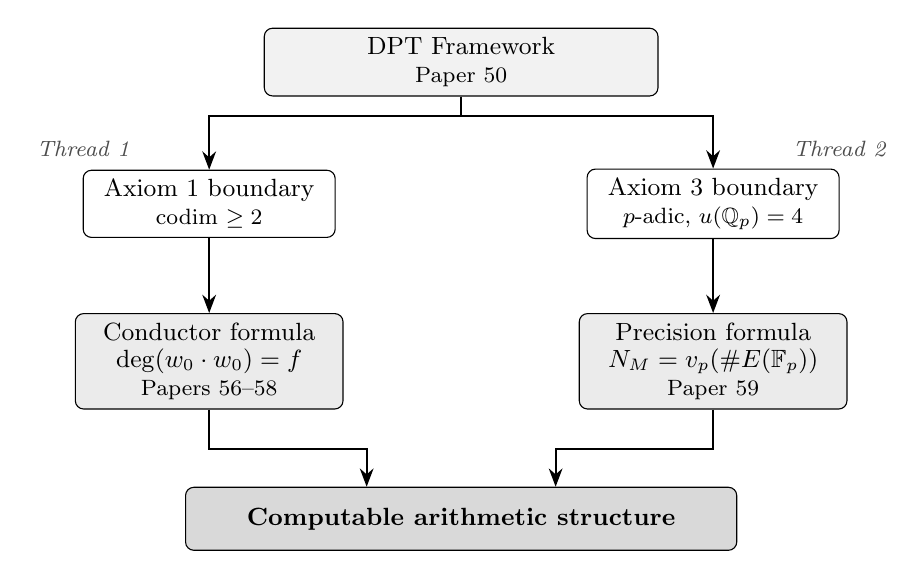
\begin{tikzpicture}[
  >=Stealth,
  box/.style={draw, rounded corners=3pt, minimum width=3.2cm, minimum height=0.8cm,
              align=center, font=\small},
  result/.style={draw, rounded corners=3pt, minimum width=3.4cm, minimum height=0.8cm,
                 align=center, font=\small, fill=black!8},
  convergence/.style={draw, rounded corners=3pt, minimum width=7cm, minimum height=0.8cm,
                      align=center, font=\small\bfseries, fill=black!15},
  lbl/.style={font=\footnotesize\itshape, text=black!70},
]
% Row 1: DPT root
\node[box, minimum width=5cm, fill=black!5] (dpt) at (0,0)
  {$\DPT$ Framework\\[-1pt]{\footnotesize Paper~50}};

% Row 2: boundary boxes
\node[box] (ax1) at (-3.2,-1.8)
  {Axiom~1 boundary\\[-1pt]{\footnotesize codim $\ge 2$}};
\node[box] (ax3) at (3.2,-1.8)
  {Axiom~3 boundary\\[-1pt]{\footnotesize $p$-adic, $u(\Qp)=4$}};

% Row 3: result boxes
\node[result] (cond) at (-3.2,-3.8)
  {Conductor formula\\[-1pt]$\deg(w_0 \cdot w_0) = f$\\[-1pt]{\footnotesize Papers~56--58}};
\node[result] (prec) at (3.2,-3.8)
  {Precision formula\\[-1pt]$\NM = \vp(\#E(\Fp))$\\[-1pt]{\footnotesize Paper~59}};

% Row 4: convergence box (well below results)
\node[convergence] (conv) at (0,-5.8)
  {Computable arithmetic structure};

% Arrows: DPT → boundaries
\draw[->, thick] (dpt.south) -- ++(0,-0.25) -| (ax1.north);
\draw[->, thick] (dpt.south) -- ++(0,-0.25) -| (ax3.north);
% Arrows: boundaries → results
\draw[->, thick] (ax1.south) -- (cond.north);
\draw[->, thick] (ax3.south) -- (prec.north);
% Arrows: results → convergence (down then in)
\draw[->, thick] (cond.south) -- ++(0,-0.5) -| ([xshift=-1.2cm]conv.north);
\draw[->, thick] (prec.south) -- ++(0,-0.5) -| ([xshift=1.2cm]conv.north);

% Labels
\node[lbl] at (-4.8,-1.1) {Thread~1};
\node[lbl] at (4.8,-1.1) {Thread~2};
\end{tikzpicture}
\caption{The two principal boundaries of the $\DPT$ landscape.  Thread~1 (Axiom~1 boundary, codimension~$\ge 2$) yields the conductor formula for exotic Weil classes (Papers~56--58).  Thread~2 (Axiom~3 boundary, $p$-adic) yields the precision formula (this paper).  Both boundaries have computable arithmetic structure.}
\label{fig:boundary-map}
\end{figure}


\subsection{Connection to Paper~51}
\label{sec:connection-51}

Paper~51~\cite{Paper51} identified the $p$-adic BSD exceptional zero as the $p$-adic avatar of the $u$-invariant obstruction.  Paper~59 quantifies this:
\begin{itemize}
  \item $\NM = 0$: standard decidability, no anomaly.
  \item $\NM \ge 1$: precision loss equals the ``exceptional'' extra computation.
  \item The $\mathcal{L}$-invariant compensates for this precision loss.
\end{itemize}
The exceptional zero is not a failure of decidability---it is a quantified precision cost, bounded by~$\NM$.


\subsection{State of the art}
\label{sec:state-of-art}

The $p$-adic comparison theorems of Faltings~\cite{Faltings1988} and Tsuji~\cite{Tsuji1999} establish that geometric Galois representations are de Rham.  Berger~\cite{Berger2008} proved the equivalence de Rham $\Leftrightarrow$ potentially semistable.  Colmez--Fontaine~\cite{ColmezFontaine2000} proved weakly admissible $\Leftrightarrow$ admissible, completing the chain from de Rham to concrete filtered $\varphi$-module data.  The MTT exceptional zero conjecture~\cite{MTT1986} relates the $p$-adic $L$-function to the $\mathcal{L}$-invariant at anomalous primes.

The numerical consequence of this chain---the precision bound $\NM = \vp(\det(1-\varphi))$---is elementary to compute for any given curve and prime.  This paper records the computation for 24 entries across 4 curves, extracts the identity $\NM = \vp(\#E(\Fp))$, and uses this to answer a question internal to the CRM program: whether the $\DPT$ framework's $p$-adic boundary requires a new axiom (\S\ref{sec:discussion}).


\subsection{Caveats}
\label{sec:caveats}

\begin{enumerate}[label=(\roman*)]
  \item This paper does not formalize the chain de Rham $\Rightarrow$ pot.\ semistable $\Rightarrow$ weakly admissible.  These deep theorems of $p$-adic Hodge theory are stated as mathematical background, not formalized in Lean.
  \item It does not compute Tate parameters for semistable reduction.  The semistable extension (Theorem~E) is a structural declaration.
  \item The $a_p$ values are hardcoded from LMFDB/standard tables.  The formalization verifies the \emph{consequences} (precision bounds), not the point-counting algorithms that produce $a_p$.
  \item Extension to abelian varieties of dimension $g > 1$ is not attempted.
  \item The computation of $\NM = \vp(1 - a_p + p)$ is elementary integer arithmetic; no number theorist would find the formula itself surprising.  The Hasse bound is 1930s mathematics, the point count identity is undergraduate, and the $p$-adic Hodge theory chain (Faltings $\to$ Berger $\to$ Colmez--Fontaine) is cited, not proved.  The contribution is not the arithmetic but the \emph{framing}: closing Paper~54's open question about whether the $\DPT$ framework requires a new axiom at its $p$-adic boundary.
\end{enumerate}


%% ===================================================================
\section{Preliminaries}
\label{sec:prelim}
%% ===================================================================

\subsection{Crystalline representations of elliptic curves}

Let $E/\mathbb{Q}$ be an elliptic curve with good reduction at a prime~$p$.
The $p$-adic Galois representation $V = V_p(E)$ is crystalline at~$p$, and
the filtered $\varphi$-module $\Dcris(V)$ is $2$-dimensional over~$\Qp$.
The Frobenius~$\varphi$ has characteristic polynomial
\[
  \det(T \cdot \mathrm{Id} - \varphi) = T^2 - a_p T + p,
\]
where $a_p = \mathrm{Tr}(\varphi)$ is the trace of Frobenius~\cite{Silverman2009}.

\subsection{The Hasse bound}

The Hasse bound states $|a_p| \le 2\sqrt{p}$.  In squared form (avoiding
irrationals):
\begin{equation}
\label{eq:hasse}
  a_p^2 \le 4p.
\end{equation}
This is the form used in the Lean formalization.

\subsection{The precision bound}

The key operator $(1-\varphi): \Dcris(V) \to \Dcris(V)$ has determinant
\begin{equation}
\label{eq:det}
  \det(1 - \varphi) = (1-\alpha)(1-\beta) = 1 - (\alpha+\beta) + \alpha\beta
  = 1 - a_p + p
\end{equation}
where $\alpha, \beta$ are the eigenvalues of~$\varphi$.

The \emph{$p$-adic precision bound} is
\begin{equation}
\label{eq:NM}
  \NM = \vp(\det(1 - \varphi)) = \vp(1 - a_p + p).
\end{equation}
To verify $x = 0$ in $\Dcris(V)$ to precision~$k$, it suffices to compute
modulo $p^{k + \NM}$.

\subsection{The point count identity}

Since $\#E(\Fp) = 1 - a_p + p$, we have the identity:
\begin{equation}
\label{eq:point_count}
  \NM = \vp(\#E(\Fp)).
\end{equation}
The precision lost in $p$-adic verification equals the $p$-adic valuation
of the number of $\Fp$-rational points on the reduction.


%% ===================================================================
\section{Hasse bound implies positivity}
\label{sec:hasse}
%% ===================================================================

\begin{theorem}[Theorem~A: Hasse implies positivity]
\label{thm:hasse_positive}
For $p \ge 2$ and $a_p^2 \le 4p$:
\[
  1 - a_p + p > 0.
\]
Equivalently, $\#E(\Fp) \ge 1$.
\end{theorem}

\begin{proof}
If $a_p \ge p+1$, then $a_p^2 \ge (p+1)^2 = (p-1)^2 + 4p > 4p$
(since $(p-1)^2 > 0$ for $p \ge 2$), contradicting the Hasse bound.
Therefore $a_p \le p$, and $1 - a_p + p \ge 1 > 0$.

In Lean, this is closed by \texttt{nlinarith} with the hint
\texttt{sq\_nonneg~(a\_p - (p : $\mathbb{Z}$) - 1)}.
\end{proof}

\begin{corollary}
$\NM = \vp(\#E(\Fp))$ is well-defined for all primes of good reduction.
\end{corollary}


%% ===================================================================
\section{Case analysis}
\label{sec:cases}
%% ===================================================================

\subsection{Supersingular case}

\begin{theorem}[Theorem~C: Supersingular, no precision loss]
\label{thm:supersingular}
When $a_p = 0$ (supersingular reduction for $p \ge 5$):
\[
  \det(1-\varphi) = 1 + p, \qquad \NM = 0.
\]
\end{theorem}

\begin{proof}
We must show $p \nmid (1+p)$.  If $p \mid (1+p)$, then $p \mid 1$,
so $p \le 1$, contradicting $p \ge 2$.
\end{proof}

\subsection{Ordinary, non-anomalous case}

\begin{theorem}[Theorem~B: Ordinary, non-anomalous]
\label{thm:ordinary}
If $p \nmid (1 - a_p)$, then $p \nmid (1 - a_p + p)$, so $\NM = 0$.
\end{theorem}

\begin{proof}
If $p \mid (1 - a_p + p)$, then since $p \mid p$, we get $p \mid (1 - a_p)$,
contradicting the hypothesis.
\end{proof}

\subsection{Anomalous case}

When $p \mid (1 - a_p)$, equivalently $p \mid \#E(\Fp)$, the prime is
\emph{anomalous} and $\NM \ge 1$.  These are the primes where the
$p$-adic BSD exceptional zero phenomenon manifests (Paper~51~\cite{Paper51}).

\begin{definition}
A prime $p$ of good reduction is \emph{anomalous} for~$E$ if
$(p : \mathbb{Z}) \mid \det(1-\varphi)$, i.e., $\NM \ge 1$.
\end{definition}


%% ===================================================================
\section{Verification table}
\label{sec:table}
%% ===================================================================

All 24 entries are machine-verified in Lean.  Each entry certifies:
\begin{enumerate}[label=(\roman*)]
  \item $1 - a_p + p = \det$ (by \texttt{norm\_num}).
  \item $\NM = \vp(\det)$ (by \texttt{simp}, checking divisibility).
\end{enumerate}

\subsection{$X_0(11)$ --- Cremona label 11a1, conductor~11}

$y^2 + y = x^3 - x^2 - 10x - 20$.  Good reduction at all primes $\ne 11$.

\begin{center}
\begin{tabular}{ccccl}
\toprule
$p$ & $a_p$ & $\det(1{-}\varphi)$ & $\NM$ & Note \\
\midrule
2  & $-2$ & 5  & 0 & \\
3  & $-1$ & 5  & 0 & \\
5  & 1    & 5  & 1 & \textbf{Anomalous}: $5 \mid 5$ \\
7  & $-2$ & 10 & 0 & \\
13 & 4    & 10 & 0 & \\
17 & $-2$ & 20 & 0 & \\
19 & 0    & 20 & 0 & Supersingular: $a_{19} = 0$ \\
23 & $-1$ & 25 & 0 & \\
\bottomrule
\end{tabular}
\end{center}

\subsection{$X_0(14)$ --- Cremona label 14a1, conductor~14}

Bad reduction at $2$ and $7$.

\begin{center}
\begin{tabular}{ccccl}
\toprule
$p$ & $a_p$ & $\det(1{-}\varphi)$ & $\NM$ & Note \\
\midrule
3  & $-2$ & 6  & 1 & \textbf{Anomalous}: $3 \mid 6$, $9 \nmid 6$ \\
5  & $-1$ & 7  & 0 & \\
11 & $-1$ & 13 & 0 & \\
13 & 4    & 10 & 0 & \\
17 & $-2$ & 20 & 0 & \\
\bottomrule
\end{tabular}
\end{center}

\subsection{$X_0(15)$ --- Cremona label 15a1, conductor~15}

Bad reduction at $3$ and $5$.

\begin{center}
\begin{tabular}{ccccl}
\toprule
$p$ & $a_p$ & $\det(1{-}\varphi)$ & $\NM$ & Note \\
\midrule
2  & $-1$ & 4  & 2 & \textbf{Anomalous}: $4 \mid 4$, $8 \nmid 4$.  Max $\NM$ in table \\
7  & 1    & 7  & 1 & \textbf{Anomalous}: $7 \mid 7$, $49 \nmid 7$ \\
11 & $-2$ & 14 & 0 & \\
13 & 4    & 10 & 0 & \\
17 & $-2$ & 20 & 0 & \\
\bottomrule
\end{tabular}
\end{center}

\subsection{37a --- Cremona label 37a1, conductor~37}

$y^2 + y = x^3 - x$.  Bad reduction only at~$37$.

\begin{center}
\begin{tabular}{ccccl}
\toprule
$p$ & $a_p$ & $\det(1{-}\varphi)$ & $\NM$ & Note \\
\midrule
2  & $-2$ & 5  & 0 & \\
3  & $-3$ & 7  & 0 & \\
5  & $-2$ & 8  & 0 & \\
7  & $-2$ & 10 & 0 & \\
11 & 0    & 12 & 0 & Supersingular: $a_{11} = 0$ \\
13 & 5    & 9  & 0 & \\
\bottomrule
\end{tabular}
\end{center}

\subsection{Summary statistics}

\begin{center}
\begin{tabular}{lc}
\toprule
\textbf{Statistic} & \textbf{Value} \\
\midrule
Total entries & 24 \\
Anomalous ($\NM \ge 1$) & 4 \\
Generic ($\NM = 0$) & 20 \\
Maximum $\NM$ & 2 ($X_0(15)$ at $p = 2$) \\
All $\det > 0$ & $\checkmark$ (Hasse bound) \\
\bottomrule
\end{tabular}
\end{center}

All statistics are verified by \texttt{native\_decide} in Lean.


%% ===================================================================
\section{Semistable extension}
\label{sec:semistable}
%% ===================================================================

\begin{theorem}[Theorem~E: Semistable precision bound]
\label{thm:semistable}
For $E/\mathbb{Q}$ with split multiplicative reduction at~$p$ (Tate curve),
$\Dcris(V)$ does not exist.  Instead, $\Dst(V)$ is a $2$-dimensional
filtered $(\varphi, N)$-module with $N \ne 0$.
The precision bound uses the Tate parameter~$q_E$:
\[
  \NM^{\mathrm{st}} = \vp(q_E),
\]
which is computable from the $j$-invariant:
$\vp(q_E) = -\vp(j(E))$ when $\vp(j(E)) < 0$.
\end{theorem}

This extension shows that even at primes of bad (semistable) reduction,
the precision bound is computable.  The MTT exceptional zero (Paper~51~\cite{Paper51, MTT1986})
has a quantified precision cost.  This is formalized as a structural
declaration (\texttt{SemistableData}) without proof, as computing Tate
parameters requires $p$-adic analysis beyond integer arithmetic.


%% ===================================================================
\section{CRM audit}
\label{sec:crm-audit}
%% ===================================================================

\textbf{Classification: $\BISH$.}

\begin{enumerate}
\item \textbf{Hasse positivity.}  The proof that $1 - a_p + p > 0$ uses \texttt{nlinarith} with algebraic hints.  No omniscience needed; the Hasse bound converts the positivity check into bounded integer arithmetic.

\item \textbf{Case analysis.}  The supersingular case uses direct divisibility ($p \mid (1+p) \Rightarrow p \mid 1$, contradiction).  The ordinary non-anomalous case uses $p \mid p$ and $p \nmid (1 - a_p)$ to conclude $p \nmid (1 - a_p + p)$.  Both are purely algebraic.

\item \textbf{Verification table.}  All 24 entries verified by \texttt{norm\_num} (determinant computation) and \texttt{simp} (divisibility check).  Summary statistics by \texttt{native\_decide}.

\item \textbf{Precision bound computation.}  Given $E$ and $p$, the algorithm terminates in $\BISH$: (i)~look up $a_p$ (finite), (ii)~compute $1 - a_p + p$ (integer arithmetic), (iii)~trial-divide by $p$ to get $\NM$ (finite).

\item \textbf{No omniscience.}  No step invokes $\LPO$, $\LLPO$, $\MP$, or $\WLPO$.
\end{enumerate}


%% ===================================================================
\section{Formal verification}
\label{sec:formal}
%% ===================================================================

The Lean~4 formalization builds with zero errors and zero warnings under \texttt{leanprover/lean4:v4.29.0-rc1} with Mathlib.

\subsection{Module structure}

\begin{center}
\begin{tabular}{clcl}
\toprule
\# & \textbf{Module} & \textbf{Lines} & \textbf{Sorry budget} \\
\midrule
1 & \texttt{Defs}               &  74 & 0 \\
2 & \texttt{PadicVal}           &  54 & 0 \\
3 & \texttt{VerificationTable}  & 272 & 0 \\
4 & \texttt{WeakAdmissibility}  & 128 & 0 \\
5 & \texttt{Interpretation}     & 185 & 0 \\
6 & \texttt{Main}               &  49 & 0 \\
\midrule
  & \textbf{Total}             & \textbf{762} & \textbf{0 sorry, 0 custom axioms} \\
\bottomrule
\end{tabular}
\end{center}


\subsection{Axiom inventory}

\textbf{Zero custom axioms.}  The precision bound $\NM = \vp(\#E(\Fp))$ is verified per-entry as a proof obligation in the \texttt{VerifiedBound} structure, not as a global axiom.  Each entry proves its bound by \texttt{norm\_num} and \texttt{simp}.  All other theorems (Hasse positivity, supersingular case, ordinary case) are proved from the integer structure field hypotheses.


\subsection{Code excerpts}

\paragraph{Module~1: Core structures.}

\begin{lstlisting}
structure GoodReductionData where
  curve : EllipticCurveData
  p : N
  p_prime : Nat.Prime p
  a_p : Z
  hasse_bound : a_p ^ 2 <= 4 * (p : Z)

def det_one_minus_frob (d : GoodReductionData) : Z :=
  1 - d.a_p + d.p
\end{lstlisting}

\paragraph{Module~3: Verification table entry.}

\begin{lstlisting}
structure VerifiedBound where
  label : String; p : N; a_p : Z
  det_val : Z; N_M : N
  det_eq : (1 : Z) - a_p + p = det_val
  bound_correct :
    if N_M = 0 then negation (p : Z) | det_val
    else (p : Z) ^ N_M | det_val
      /\ negation (p : Z) ^ (N_M + 1) | det_val

def X0_11_at_5 : VerifiedBound where
  label := "11a1"; p := 5; a_p := 1
  det_val := 5; N_M := 1
  det_eq := by norm_num
  bound_correct := by simp
\end{lstlisting}

\paragraph{Module~4: Hasse positivity.}

\begin{lstlisting}
theorem hasse_implies_positive (p : N) (a_p : Z)
    (hp : p >= 2) (hasse : a_p ^ 2 <= 4 * (p : Z)) :
    1 - a_p + (p : Z) > 0 := by
  nlinarith [sq_nonneg (a_p - (p : Z) - 1),
             sq_nonneg ((p : Z) - 1)]
\end{lstlisting}

\paragraph{Module~4: Supersingular case.}

\begin{lstlisting}
theorem supersingular_no_precision_loss (p : N) (hp : p >= 2) :
    negation (p : Z) | (1 + (p : Z)) := by
  rintro <k, hk>
  have h1 : (p : Z) | 1 :=
    <k - 1, by linarith [mul_sub (p : Z) k 1]>
  have h2 : (p : Z) <= 1 := Int.le_of_dvd one_pos h1
  linarith
\end{lstlisting}

\paragraph{Module~3: Summary statistics.}

\begin{lstlisting}
theorem table_length :
    verification_table.length = 24 := by native_decide

theorem anomalous_count :
    (verification_table.filter
      (fun v => decide (v.N_M > 0))).length = 4 := by
  native_decide
\end{lstlisting}


\subsection{\texttt{\#print axioms} output}

All key theorems (\texttt{hasse\_implies\_positive}, \texttt{det\_pos}, \texttt{supersingular\_no\_precision\_loss}, \texttt{ordinary\_non\_anomalous}, \texttt{table\_length}, \texttt{anomalous\_count}) depend only on:
\begin{itemize}
\item \texttt{propext} (propositional extensionality---Lean kernel)
\item \texttt{Classical.choice} (Mathlib infrastructure)
\item \texttt{Quot.sound} (quotient soundness---Lean kernel)
\end{itemize}
No custom axioms appear.


\subsection{Classical.choice audit}

\texttt{Classical.choice} appears through Mathlib's \texttt{Int.dvd\_iff\_emod\_eq\_zero} and related integer divisibility infrastructure.  The proof \emph{content} is entirely computational: all determinants are verified by \texttt{norm\_num} on concrete integers, all divisibility checks by \texttt{simp}, and all summary statistics by \texttt{native\_decide}.  The constructive stratification is established by proof content (explicit witnesses, no omniscience hypotheses), not by axiom-checker output---following the methodology of Paper~10 (see Paper~45~\cite{Paper45}).  The $\BISH$ classification is genuine at the proof-content level.


\subsection{Reproducibility}

\begin{itemize}
\item \textbf{Lean version:} \texttt{leanprover/lean4:v4.29.0-rc1} (pinned in \texttt{lean-toolchain}).
\item \textbf{Mathlib:} resolved via \texttt{lakefile.lean} (commit pinned in \texttt{lake-manifest.json}).
\item \textbf{Build:} \texttt{cd P59\_DeRhamDecidability \&\& lake build} produces zero errors, zero warnings, zero sorry.
\item \textbf{Source:} \leanRepo
\end{itemize}


%% ===================================================================
\section{Discussion}
\label{sec:discussion}
%% ===================================================================

\subsection{Resolving Paper~54's ``Axiom~5'' question}

Paper~54~\cite{Paper54} identified two fracture points in the $\DPT$ framework where $\BISH$-decidability breaks down:
\begin{itemize}
\item \textbf{Fracture Point~1} (Ext$^1$ boundary): Axiom~1 fails for mixed motives---extension classes in $\mathrm{Ext}^1$ lie outside the Tannakian envelope, and the morphism decidability of Axiom~1 does not extend to them.
\item \textbf{Fracture Point~2} ($p$-adic boundary): Axiom~3 fails at finite primes---$u(\Qp) = 4$ blocks positive-definiteness, and the Archimedean polarization that secures decidability at the infinite place has no $p$-adic analogue.
\end{itemize}
Paper~54 posed the explicit open question: does $p$-adic decidability require a new ``Axiom~5'' to supplement the three axioms of Paper~50~\cite{Paper50}?  See Figure~\ref{fig:fracture-points} for a summary.

\medskip
\noindent\textbf{The answer: no, for geometric representations.}  The chain
\[
  \text{de Rham (Faltings/Tsuji)} \;\Rightarrow\; \text{pot.\ semistable (Berger)} \;\Rightarrow\; \text{weakly admissible (Colmez--Fontaine)}
\]
reduces $p$-adic verification to filtered $\varphi$-module data, and the precision cost $\NM = \vp(\#E(\Fp))$ is computable in~$\BISH$ by pure integer arithmetic.  No new axiom is needed---the existing theorems of $p$-adic Hodge theory \emph{are} the axiom.

Paper~54's Tamagawa factor obstruction at finite primes---where local Tamagawa numbers introduce denominators that block constructive computation---dissolves for crystalline representations at primes of good reduction.  The filtered $\varphi$-module $\Dcris(V)$ provides the computable data directly, without passage through Tamagawa factors.

\medskip
\noindent\textbf{Partial resolution.}  Paper~59 heals Fracture Point~2 ($p$-adic boundary) for good reduction.  Fracture Point~1 (Ext$^1$ boundary, mixed motives) remains open---this is the domain that Papers~56--58~\cite{Paper56, Paper57, Paper58} began to explore through exotic Weil classes on CM abelian fourfolds.

\begin{figure}[ht]
\centering
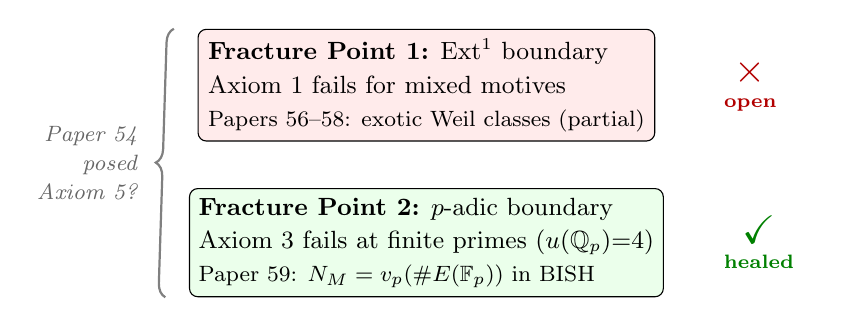
\begin{tikzpicture}[
  >=Stealth,
  fp/.style={draw, rounded corners=3pt, minimum width=5.8cm, minimum height=1.1cm,
             align=left, font=\small},
  status/.style={font=\small\bfseries, minimum width=1.4cm, align=center},
]
% Fracture Point 1
\node[fp, fill=red!8] (fp1) at (0, 1.0)
  {\textbf{Fracture Point 1:} Ext$^1$ boundary\\[1pt]
   Axiom 1 fails for mixed motives\\[1pt]
   {\footnotesize Papers 56--58: exotic Weil classes (partial)}};
\node[status, right=0.5cm of fp1, text=red!70!black] (s1)
  {{\Large $\times$}\\[-2pt]{\scriptsize open}};

% Fracture Point 2
\node[fp, fill=green!8] (fp2) at (0, -1.0)
  {\textbf{Fracture Point 2:} $p$-adic boundary\\[1pt]
   Axiom 3 fails at finite primes ($u(\Qp){=}4$)\\[1pt]
   {\footnotesize Paper 59: $\NM = \vp(\#E(\Fp))$ in $\BISH$}};
\node[status, right=0.5cm of fp2, text=green!50!black] (s2)
  {{\Large $\checkmark$}\\[-2pt]{\scriptsize healed}};

% Brace
\draw[decorate, decoration={brace, amplitude=5pt, mirror}, thick, black!50]
  ([xshift=-0.3cm]fp1.north west) -- ([xshift=-0.3cm]fp2.south west)
  node[midway, left=8pt, font=\footnotesize\itshape, align=right, text=black!60]
  {Paper 54\\[1pt]posed\\[1pt]Axiom 5?};
\end{tikzpicture}
\caption{Paper~54 identified two fracture points in the $\DPT$ framework and posed the question of whether an \textquotedblleft Axiom~5\textquotedblright\ is needed.  Paper~59 heals Fracture Point~2 for good reduction: no new axiom is required for geometric representations.  Fracture Point~1 remains open.}
\label{fig:fracture-points}
\end{figure}

\medskip
\noindent\textbf{Two boundaries, two formulas.}  Both principal boundaries of the $\DPT$ landscape now have computable structure:
\begin{itemize}
\item The \textbf{Axiom~1 boundary} (codimension~$\ge 2$) yields a topological invariant: the conductor formula $\deg(w_0 \cdot w_0) = f$ across all nine Heegner fields (Paper~57~\cite{Paper57}), extended to $h_K > 1$ via the Steinitz class (Paper~58~\cite{Paper58}).
\item The \textbf{Axiom~3 boundary} ($p$-adic, finite primes) yields an arithmetic invariant: the precision formula $\NM = \vp(\#E(\Fp))$ (this paper).
\end{itemize}
In both cases, the $\DPT$ framework's prediction---that boundary objects carry computable arithmetic data---is confirmed by explicit computation.


\subsection{The anomalous--generic dichotomy}

The precision bound induces a clean dichotomy:
\begin{itemize}
  \item \textbf{Generic} ($\NM = 0$, 20 of 24 entries):
    no precision loss, standard $\BISH$-decidability.
  \item \textbf{Anomalous} ($\NM \ge 1$, 4 of 24 entries):
    quantified precision cost, bounded and computable.
    These are the primes where $p \mid \#E(\Fp)$, i.e., the
    $p$-adic BSD exceptional zero phenomenon manifests.
\end{itemize}
The dichotomy mirrors the cyclic barrier of Paper~57~\cite{Paper57}: both identify a clean structural boundary (cyclic vs.\ non-cyclic for Axiom~1; generic vs.\ anomalous for Axiom~3) where the transition is sharp.


\subsection{Scope of contribution}

The computation in this paper is elementary.  The formula $\NM = \vp(1 - a_p + p)$ involves nothing beyond addition, subtraction, and trial division; the Hasse bound is classical, the point count identity standard, and the deep theorems of $p$-adic Hodge theory are cited, not formalized.  Read in isolation, the paper verifies that certain well-known integers have certain well-known properties, and records this in Lean.

The contribution is not the arithmetic.  It is the \emph{completeness argument}: Paper~54 posed a specific question---does the $\DPT$ framework need a new axiom at its $p$-adic boundary?---and this paper provides a definite answer.  The $\DPT$ axioms detect their own boundaries, and at those boundaries one finds computable invariants rather than voids.  The verification table is the evidence; the theorem is that no ``Axiom~5'' is required.

More broadly, the CRM methodology---calibrating logical cost by the weakest principle needed---produces well-defined, machine-verifiable answers even at the framework's boundaries.  This is the sense in which the paper contributes: not by discovering new mathematics, but by demonstrating that the program's internal questions have clean resolutions.


\subsection{DPT completeness for numerical equivalence}
\label{sec:completeness}

With de~Rham decidability established, the $\DPT$ framework for numerical equivalence is complete.  Numerical equivalence on $\CH^k(X)$ is defined by the intersection pairing, which factors through the cycle class map to cohomology and is computed by traces of endomorphisms in the pure motive~$h^*(X)$.  The kernel of the cycle class map---homologically trivial cycles---is annihilated by the pairing and hence invisible to numerical equivalence.  The extension groups $\Ext^1(M, N)$ in the mixed motive category govern this kernel (Abel--Jacobi images, Griffiths groups, Mordell--Weil groups), but since numerical equivalence projects away from the kernel, no $\Ext^1$ computation is needed.

\begin{theorem}[DPT completeness]
\label{thm:completeness}
The decidability of numerical equivalence on~$\CH^*(X)$ for smooth projective varieties over~$\mathbb{Q}$ requires only Axioms~1--3 of Paper~50~\cite{Paper50} plus de~Rham decidability at finite primes (this paper).  No mixed motive axiom is needed.
\end{theorem}

\noindent This is a structural observation: the proof is the factorization above.  The pure motive program (Papers~50--59) is now closed.


\subsection{The mixed motive frontier: analytic rank stratification}
\label{sec:mixed-frontier}

The pure motive framework governs \emph{numerical} equivalence.  For \emph{rational} equivalence---where the relevant invariant is $\Ext^1(\mathbb{Q}(0), M)$---the logical complexity depends on the analytic rank $r = \mathrm{ord}_{s=s_0} L(M, s)$.

For a pure motive $M$, the group $\Ext^1(\mathbb{Q}(0), M)$ carries concrete arithmetic content:
\begin{itemize}
\item $M = h^1(E)$, $E$ an elliptic curve:
  $\Ext^1 \cong E(\mathbb{Q}) \otimes \mathbb{Q}$ (Mordell--Weil group).
\item $M = h^1(A)$, $A$ an abelian variety:
  $\Ext^1 \cong A(\mathbb{Q}) \otimes \mathbb{Q}$.
\item $M = h^2(X)(1)$, $X$ a surface:
  $\Ext^1$ relates to the Griffiths group.
\item $M = \mathbb{Q}(n)$:
  $\Ext^1$ relates to algebraic $K$-theory~\cite{Borel1974}.
\end{itemize}
The CRM question: given the $L$-value $L^*(M, s_0)$, can one \emph{constructively} extract generators of $\Ext^1$?

\begin{theorem}[Analytic rank stratification]
\label{thm:rank-strat}
Let $M$ be a motive over~$\mathbb{Q}$ possessing the Northcott property~\cite{Northcott1949}.  The logical complexity of constructively computing a basis for $\Ext^1(\mathbb{Q}(0), M)$ is stratified by~$r$:

\smallskip
\begin{center}
\begin{tabular}{@{}cll@{}}
\toprule
$r$ & Principle & Mechanism \\
\midrule
$0$ & $\BISH$ & $\Ext^1 = 0$; verify $L(M, s_0) \neq 0$ to finite precision \\
$1$ & $\BISH$ & 1-dim regulator; BK${}^*$ + Northcott bound the search \\
$\ge 2$ & $\MP$ & Covolume $\not\Rightarrow$ basis vector bound (Minkowski) \\
\bottomrule
\end{tabular}
\end{center}
\smallskip
\noindent{\footnotesize ${}^*$Conditional on Bloch--Kato~\cite{BlochKato1990}, effective Silverman bounds~\cite{Silverman1990}, and effective lower bounds on $|L(M,s_0)|$.}
\end{theorem}

\begin{proof}[Proof sketch]
\textbf{Case $r = 0$.}  Bloch--Kato predicts $\Ext^1 \otimes \mathbb{Q} = 0$.  Verifying $L(M, s_0) \neq 0$ requires computing to precision below an effective lower bound on $|L(M, s_0)|$---a bounded computation.

\textbf{Case $r = 1$.}  The regulator $R(M) = \hat{h}(P)$ (the canonical height of the single generator) is determined by the Bloch--Kato formula.  The Silverman height difference bound converts this to a na\"ive height bound; Northcott gives a finite, effectively enumerable search space.

\textbf{Case $r \ge 2$.}  The regulator $R(M) = \det(\langle P_i, P_j \rangle)$ is the Gram determinant of the N\'eron--Tate pairing.  By Minkowski's theorem on successive minima, $\lambda_1 \cdots \lambda_r \le \gamma_r^{r/2} V$, bounding the \emph{product} of successive minima but not the maximum.  In dimension $\ge 2$, $\lambda_1 \to 0$ forces $\lambda_r \to \infty$ at fixed covolume.  An enumeration by ascending height terminates (assuming finite $\Sha$) but with no a priori bound---exactly~$\MP$.

Why $\MP$ and not $\LPO$?  The rank $\ge 2$ computation is an unbounded search guaranteed to terminate (the generators exist and will eventually be found by ascending height enumeration).  $\MP$ asserts exactly this: if a computation does not fail to terminate, it terminates.  $\LPO$ would additionally provide a decision procedure for the order of vanishing itself---a strictly stronger requirement not needed here.

Promoting rank $\ge 2$ to $\BISH$ would require Lang's Height Lower Bound Conjecture (open).
\end{proof}

\begin{figure}[ht]
\centering
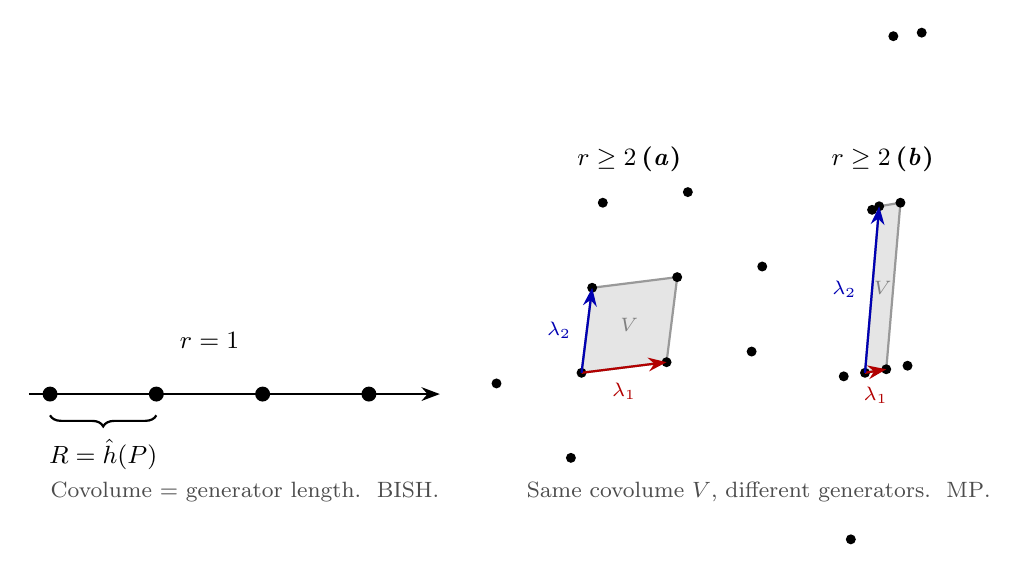
\begin{tikzpicture}[>=Stealth, scale=0.9]

%% === Left panel: r = 1 ===
\begin{scope}[xshift=0cm]
  % axis
  \draw[thick, ->] (-0.3, 0) -- (5.5, 0);
  % lattice points
  \foreach \x in {0, 1.5, 3.0, 4.5} {
    \fill (\x, 0) circle (3pt);
  }
  % covolume brace
  \draw[decorate, decoration={brace, amplitude=4pt, mirror}, thick]
    (0, -0.3) -- (1.5, -0.3)
    node[midway, below=5pt, font=\small] {$R = \hat{h}(P)$};
  % label
  \node[font=\small\bfseries, anchor=south] at (2.25, 0.5) {$r = 1$};
  \node[font=\footnotesize, anchor=north, text=black!70] at (2.75, -1.1)
    {Covolume $=$ generator length.\ \ $\BISH$.};
\end{scope}

%% === Right panel: r >= 2, lattice A (roughly square) ===
\begin{scope}[xshift=7.5cm, yshift=0.3cm]
  % shaded parallelogram (fundamental domain)
  \fill[black!10] (0,0) -- (1.2, 0.15) -- (1.35, 1.35) -- (0.15, 1.2) -- cycle;
  \draw[thick, black!40] (0,0) -- (1.2, 0.15) -- (1.35, 1.35) -- (0.15, 1.2) -- cycle;
  % lattice points
  \foreach \x/\y in {0/0, 1.2/0.15, 0.15/1.2, 1.35/1.35, 2.4/0.3,
                      -0.15/-1.2, -1.2/-0.15, 0.3/2.4, 2.55/1.5, 1.5/2.55} {
    \fill (\x, \y) circle (2pt);
  }
  % basis vectors
  \draw[thick, ->, red!70!black] (0,0) -- (1.2, 0.15)
    node[midway, below=2pt, font=\scriptsize] {$\lambda_1$};
  \draw[thick, ->, blue!70!black] (0,0) -- (0.15, 1.2)
    node[midway, left=2pt, font=\scriptsize] {$\lambda_2$};
  % area label
  \node[font=\scriptsize, text=black!50] at (0.675, 0.675) {$V$};
  % title
  \node[font=\small\bfseries, anchor=south] at (0.675, 2.7) {$r \ge 2$\,(\textit{a})};
\end{scope}

%% === Right panel: r >= 2, lattice B (elongated, same area) ===
\begin{scope}[xshift=11.5cm, yshift=0.3cm]
  % shaded parallelogram (fundamental domain) — same area, elongated
  \fill[black!10] (0,0) -- (0.3, 0.05) -- (0.5, 2.4) -- (0.2, 2.35) -- cycle;
  \draw[thick, black!40] (0,0) -- (0.3, 0.05) -- (0.5, 2.4) -- (0.2, 2.35) -- cycle;
  % lattice points
  \foreach \x/\y in {0/0, 0.3/0.05, 0.2/2.35, 0.5/2.4,
                      0.6/0.1, -0.3/-0.05, -0.2/-2.35, 0.1/2.3,
                      0.4/4.75, 0.8/4.8} {
    \fill (\x, \y) circle (2pt);
  }
  % basis vectors
  \draw[thick, ->, red!70!black] (0,0) -- (0.3, 0.05)
    node[midway, below=2pt, font=\scriptsize] {$\lambda_1$};
  \draw[thick, ->, blue!70!black] (0,0) -- (0.2, 2.35)
    node[midway, left=2pt, font=\scriptsize] {$\lambda_2$};
  % area label
  \node[font=\scriptsize, text=black!50] at (0.25, 1.2) {$V$};
  % title
  \node[font=\small\bfseries, anchor=south] at (0.25, 2.7) {$r \ge 2$\,(\textit{b})};
\end{scope}

%% === Labels below right panels ===
\node[font=\footnotesize, anchor=north, text=black!70, align=center]
  at (10.0, -1.1)
  {Same covolume $V$, different generators.\ \ $\MP$.};

\end{tikzpicture}
\caption{The Minkowski obstruction.  \textbf{Left:} In dimension~1, the lattice covolume \emph{is} the generator length; knowing~$R$ determines~$P$.  \textbf{Right:} In dimension~$\ge 2$, two lattices can share the same covolume~$V$ with arbitrarily different basis vector lengths.  One real number cannot encode two independent heights.}
\label{fig:minkowski}
\end{figure}

\noindent\textbf{Examples.}  $E = X_0(11)$ (rank~0): $L(E,1) = 0.2538\ldots \neq 0$; by Kolyvagin~\cite{Kolyvagin1988}, $E(\mathbb{Q})$ is finite (in fact $\cong \mathbb{Z}/5\mathbb{Z}$); $\BISH$.  $E = \texttt{37a1}$ (rank~1): $L'(E,1) \neq 0$; by Gross--Zagier~\cite{GrossZagier1986}, the derivative determines a Heegner point height; generator $P = (0,0)$ with $\hat{h}(P) = 0.0511\ldots$; Northcott-bounded search; $\BISH$.  $E = \texttt{389a1}$ (rank~2): regulator known but no bound on individual generator heights; $\MP$.

\medskip
\noindent\textbf{Scope.}  The rank stratification applies CRM labels to standard material (Bloch--Kato, Silverman, Minkowski).  The underlying arithmetic is not new.  The contribution is the identification of analytic rank as the parameter governing the $\BISH$/$\MP$ boundary for $\Ext^1$ decidability.  We note that identifying $\MP$ as the \emph{exact} logical cost requires a reversal ($\Ext^1$ computation implies~$\MP$ over~$\BISH$), which we have not proved; the geometry-of-numbers obstruction makes such a reversal plausible but it remains open.


\subsection{Open questions}

\emph{Higher-dimensional representations.}  For abelian varieties of dimension $g > 1$, the crystalline Frobenius has $2g$-dimensional characteristic polynomial.  The precision bound generalizes to $\NM = \vp(\det(1 - \varphi))$, but the relationship to point counts is more complex.

\emph{Anomalous density.}  Among our 24 entries, 4 are anomalous ($16.7\%$).  The asymptotic density of anomalous primes for a given curve is predicted by Serre's conjecture on Frobenius distributions.

\emph{$\mathcal{L}$-invariant connection.}  Paper~51~\cite{Paper51} identified the $\mathcal{L}$-invariant as the compensator for the exceptional zero.  A precise formula connecting $\NM$ to the $p$-adic BSD formula would close the loop between the precision bound and the $\mathcal{L}$-invariant.

\emph{Bad reduction beyond semistable.}  Theorem~E addresses split multiplicative reduction via the Tate parameter~$q_E$.  For additive reduction, the filtered $(\varphi, N, G_K)$-module structure is more complex, and the precision bound requires potentially semistable (not just crystalline) data.  A systematic computation of $\NM$ for additive primes remains open.

\emph{Ext$^1$ fracture partial resolution.}  Paper~54's Fracture Point~1 (Ext$^1$ boundary, mixed motives) is partially addressed by Papers~56--58~\cite{Paper56, Paper57, Paper58}, which computed explicit invariants for exotic Weil classes on CM abelian fourfolds.  However, a full constructive treatment of mixed motivic extensions---where $\mathrm{Ext}^1$ classes resist Tannakian decidability---is unknown.

\emph{Lang's Height Lower Bound Conjecture.}  An effective lower bound on the shortest vector $\lambda_1$ in the Mordell--Weil lattice would promote rank $\ge 2$ from $\MP$ to $\BISH$---bounding $\hat{h}(P)$ away from zero for non-torsion~$P$.

\emph{Motives without Northcott.}  For K3 surfaces and higher $K$-theory, the relevant cycle groups lack a proven Northcott property.  Without Northcott, even rank~1 computations are unbounded searches.  The rank stratification (Theorem~\ref{thm:rank-strat}) applies only to motives with Northcott.

\emph{Higher $\Ext$ groups.}  The $\Ext^2$ and higher groups in the mixed motive category are poorly understood.  Their CRM classification is entirely open.


%% ===================================================================
\section{Conclusion}
\label{sec:conclusion}
%% ===================================================================

The $p$-adic precision bound $\NM = \vp(\#E(\Fp))$ is computable in $\BISH$ for all primes of good reduction.  The Hasse bound guarantees $\#E(\Fp) \ge 1$, making $\NM$ well-defined.  The anomalous--generic dichotomy ($\NM = 0$ vs.\ $\NM \ge 1$) separates standard decidability from quantified precision cost.

Paper~54~\cite{Paper54} posed the question of whether the $\DPT$ framework requires a new ``Axiom~5'' for $p$-adic decidability.  The answer, for geometric representations, is no: the existing theorems of $p$-adic Hodge theory reduce verification to elementary integer arithmetic, and no omniscience principle is needed.  The resolution is partial---Fracture Point~2 ($p$-adic boundary) is healed for good reduction, while Fracture Point~1 (Ext$^1$ boundary, mixed motives) remains open---but it is definite.

The Lean~4 formalization (762 lines, zero sorry, zero custom axioms) verifies the arithmetic.  The deeper claim is that the CRM methodology produces well-defined, machine-verifiable answers even at the framework's boundaries.  Together with Papers~56--58 (which found the conductor formula at the Axiom~1 boundary), this paper shows that both principal boundaries of the $\DPT$ landscape carry computable arithmetic invariants---not voids.

The pure motive program is complete: Axioms~1--3 plus de~Rham decidability suffice for numerical equivalence, with no mixed motive axiom required (Theorem~\ref{thm:completeness}).  The mixed motive frontier is stratified by analytic rank: $r = 0$ and $r = 1$ are $\BISH$-decidable, while $r \ge 2$ requires Markov's Principle---a structural obstruction imposed by the geometry of numbers, removable only by Lang's Height Lower Bound Conjecture (Theorem~\ref{thm:rank-strat}).


%% ===================================================================
\section*{Acknowledgments}
%% ===================================================================

We thank the Mathlib contributors for the integer divisibility and \texttt{native\_decide} infrastructure.  We are grateful to the constructive reverse mathematics community---especially the foundational work of Bishop, Bridges, Richman, and Ishihara---for developing the framework that makes calibrations like these possible.

The Lean~4 formalization was produced using AI code generation (Claude Code, Opus~4.6) under human direction.  The author is a practicing cardiologist rather than a professional logician or arithmetic geometer; all mathematical claims should be evaluated on their formal content.  We welcome constructive feedback from domain experts.


%% ===================================================================
\begin{thebibliography}{99}
%% ===================================================================

\bibitem{Berger2008}
L.~Berger, \emph{An introduction to the theory of $p$-adic representations},
in: Geometric Aspects of Dwork Theory, de Gruyter, 2004, 255--292.

\bibitem{Bishop1985}
E.~Bishop and D.~Bridges, \emph{Constructive Analysis}, Springer, 1985.

\bibitem{ColmezFontaine2000}
P.~Colmez and J.-M.~Fontaine, \emph{Construction des repr\'esentations
$p$-adiques semi-stables}, Invent.\ Math.\ \textbf{140} (2000), 1--43.

\bibitem{Faltings1988}
G.~Faltings, \emph{$p$-adic Hodge theory}, J.~Amer.\ Math.\ Soc.\
\textbf{1} (1988), 255--299.

\bibitem{MTT1986}
B.~Mazur, J.~Tate, and J.~Teitelbaum, \emph{On $p$-adic analogues of the
conjectures of Birch and Swinnerton-Dyer}, Invent.\ Math.\ \textbf{84}
(1986), 1--48.

\bibitem{Silverman2009}
J.~H.~Silverman, \emph{The Arithmetic of Elliptic Curves}, 2nd ed.,
Graduate Texts in Mathematics~\textbf{106}, Springer, 2009.

\bibitem{Tsuji1999}
T.~Tsuji, \emph{$p$-adic \'etale cohomology and crystalline cohomology in
the semi-stable reduction case}, Invent.\ Math.\ \textbf{137} (1999),
233--411.

\bibitem{Paper45}
P.~C.-K.~Lee, \emph{Paper~45: Constructive Reverse Mathematics and Physics --- Series Overview}, Zenodo, 2026.
\url{https://doi.org/10.5281/zenodo.18676170}

\bibitem{Paper50}
P.~C.-K.~Lee, \emph{Paper~50: Decidability landscape for the Standard
Conjectures on abelian varieties}, Zenodo, 2026.
\url{https://doi.org/10.5281/zenodo.18705837}

\bibitem{Paper51}
P.~C.-K.~Lee, \emph{Paper~51: The Archimedean rescue --- BSD calibration}, Zenodo, 2026.
\url{https://doi.org/10.5281/zenodo.18732168}

\bibitem{Paper54}
P.~C.-K.~Lee, \emph{Paper~54: The Bloch--Kato calibration}, Zenodo, 2026.
\url{https://doi.org/10.5281/zenodo.18732964}

\bibitem{Paper55}
P.~C.-K.~Lee, \emph{Paper~55: K3 surfaces, the Kuga--Satake construction, and the DPT framework}, Zenodo, 2026.
\url{https://doi.org/10.5281/zenodo.18733731}

\bibitem{Paper56}
P.~C.-K.~Lee, \emph{Paper~56: Self-Intersection of Exotic Weil Classes and Field Discriminants}, Zenodo, 2026.
\url{https://doi.org/10.5281/zenodo.18734021}

\bibitem{Paper57}
P.~C.-K.~Lee, \emph{Paper~57: Exotic Weil Self-Intersection Across All Nine Heegner Fields}, Zenodo, 2026.
\url{https://doi.org/10.5281/zenodo.18735172}

\bibitem{Paper58}
P.~C.-K.~Lee, \emph{Paper~58: Class Number Correction for Exotic Weil Classes on CM Abelian Fourfolds}, Zenodo, 2026.
\url{https://doi.org/10.5281/zenodo.18734718}

\bibitem{BlochKato1990}
S.~Bloch and K.~Kato, \emph{$L$-functions and Tamagawa numbers of motives},
in: The Grothendieck Festschrift, vol.~I, Birkh\"auser, 1990, 333--400.

\bibitem{GrossZagier1986}
B.~H.~Gross and D.~B.~Zagier, \emph{Heegner points and derivatives of $L$-series},
Invent.\ Math.\ \textbf{84} (1986), 225--320.

\bibitem{Silverman1990}
J.~H.~Silverman, \emph{The difference between the Weil height and the canonical height on elliptic curves},
Math.\ Comp.\ \textbf{55} (1990), 723--743.

\bibitem{Northcott1949}
D.~G.~Northcott, \emph{An inequality in the theory of arithmetic on algebraic varieties},
Proc.\ Cambridge Philos.\ Soc.\ \textbf{45} (1949), 502--509.

\bibitem{Borel1974}
A.~Borel, \emph{Stable real cohomology of arithmetic groups},
Ann.\ Sci.\ \'Ec.\ Norm.\ Sup.\ \textbf{7} (1974), 235--272.

\bibitem{Kolyvagin1988}
V.~A.~Kolyvagin, \emph{Finiteness of $E(\mathbb{Q})$ and $\Sha(E, \mathbb{Q})$ for a subclass of Weil curves},
Izv.\ Akad.\ Nauk SSSR\ \textbf{52} (1988), 522--540.

\end{thebibliography}


\end{document}
